\chapter{Controller Design}\label{chap:Control}
The quadcopter system has been described with multiple mathematical models, for both the attitude and the translational behavior, these can be found in \autoref{chap:Model}. These models are utilized when designing the different controllers. The controllers are designed to fulfil the relevant functional requirements stated in \autoref{ch:functionalRequirements}.

The model is divided into two submodels, an attitude model and a translational model. It is therefore desirable to design two control systems, one for each subsystem. \autoref{fig:ControlHeadDiagram} shows the relation between the different controllers and models in the system.

% The attitude controller constitutes the inner loop, which is surrounded by the x and y translational controllers. An z controller, separated from attitude controller, handles the amount of thrust applied by the motors, by changing the required sum of their rotational speeds. 
%
\begin{figure}[H]
	\centering
	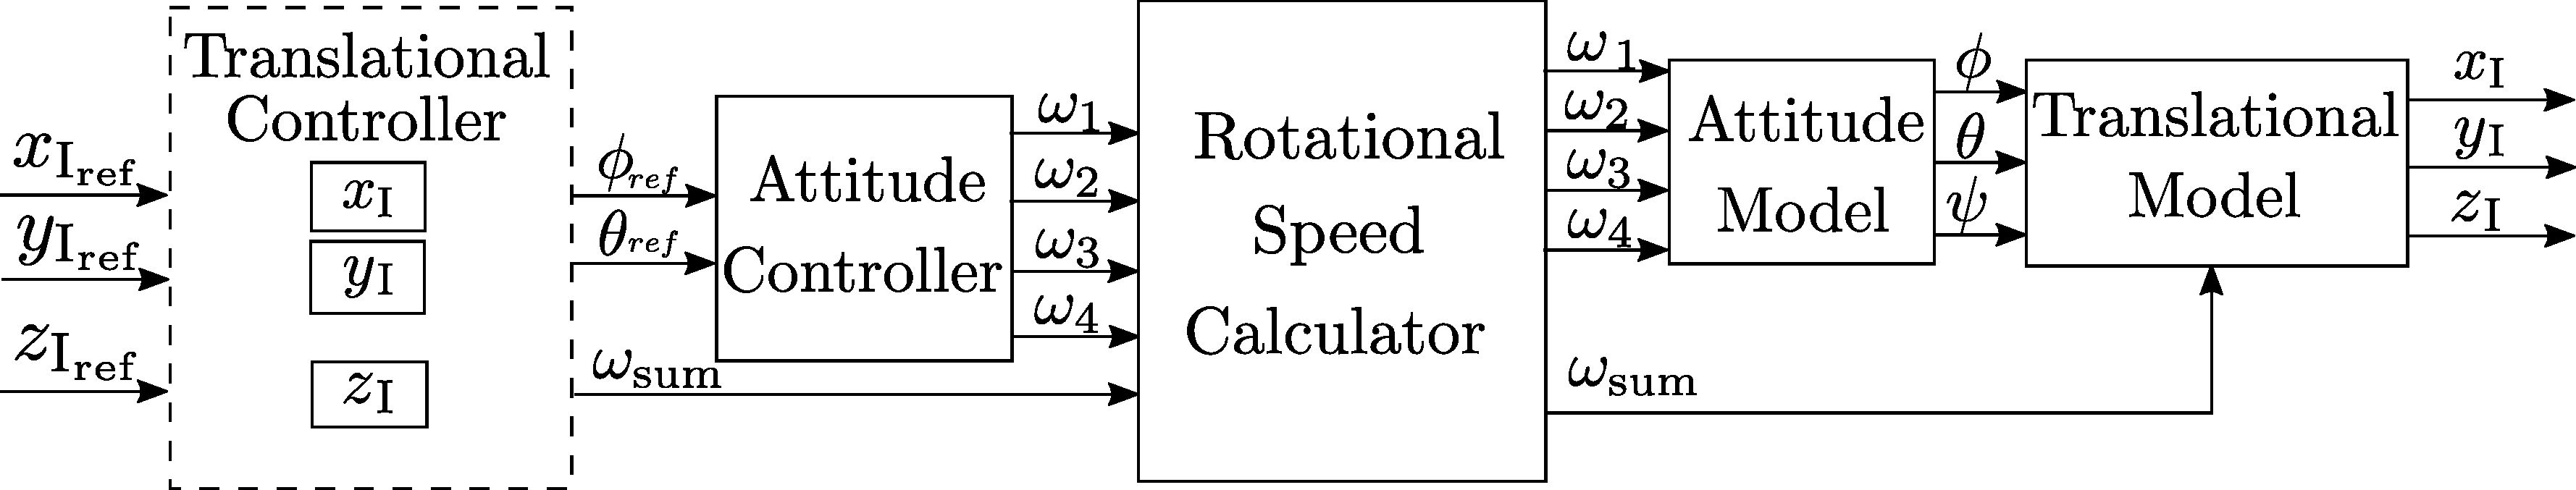
\includegraphics[width=1 \textwidth]{figures/generalcontroldiagram2}
	\caption{Block diagram of the overall control system.}
	\label{fig:ControlHeadDiagram}
\end{figure}
%
The translational controller, inertial position in $x$ ($x\mathrm{_I}$), inertial position in $y$ ($y\mathrm{_I}$) and inertial position in $z$ ($z\mathrm{_I}$), are designed with classical control methods. This control block receives the desired $x_\mathrm{I_{ref}}$, $y_\mathrm{I_{ref}}$ and $z_\mathrm{I_{ref}}$ positions. The translational controllers for $x\mathrm{_I}$ and $y\mathrm{_I}$ constitutes an outer loop with the attitude controller as the inner loop. The $x\mathrm{_I}$ and $y\mathrm{_I}$ translational controller passes a roll and pitch reference to the attitude controller, as these are use to change the position. Note that a reference for yaw is not illustrated on the diagram, as the attitude controller is designed to always strive for a yaw of zero. The attitude controller is designed using a state space approach \cite{ssReference}. The $z\mathrm{_I}$ controller, separated from attitude controller, handles the amount of thrust applied by the motors, by changing the required sum of their rotational speeds.

The rotational speed calculator receives the total speed of each motor and the required sum needed to get the desired thrust for the $z\mathrm{_I}$ direction. The rotational speed calculator's objective is to combine it's five inputs into four new motor velocities affecting both the attitude and the translational model. Since the difference in motor velocities affects the attitude of the quadcopter, and both the sum of the motor velocities and the attitude affects the translational model.

%takes into account the rotational speeds that the attitude controller needs in each motor and the sum that is needed to get the desired thrust in the $z_\mathrm{I}$ direction. Then, it combines both to give the final control action that is applied to the system.

This chapters starts by designing the attitude controller followed by the design of the translational controller. When the controllers are designed, they are simulated together with the model and the maximum expected delay. This is to ensure the controllers yield the desired behavior with the delay. After the design and simulations of each controller, they are discretized. The discrete controllers are simulated and compared to the simulations of the continuous controllers. This is necessary as some design considerations may be lost in the discretization. Lastly an overview of the implementation of the controllers on the micro processor is presented. 

\fxnote{write about sampling time.}